%%%%%%%%%%%%%%%%%%%%%%%%%%%%%%%%%%%%%%%%%%%%%%%%%
% PROGRAMMER: Pierre-Antoine Ksinant            %
% CREATION DATE: 05/07/2019                     %
% REVISION DATE: -                              %
% PURPOSE: Machine Learning Engineer Nanodegree %
%%%%%%%%%%%%%%%%%%%%%%%%%%%%%%%%%%%%%%%%%%%%%%%%%


%%%%%%%%%%%%%%%%%%%%%%%%%%%%%%%%%%%%%%%%%%%%%%%%%
%                   PREAMBLE                    %
%%%%%%%%%%%%%%%%%%%%%%%%%%%%%%%%%%%%%%%%%%%%%%%%%

%% Document class %%
\documentclass[twocolumn, switch]{article}

%% Personal style %%
\usepackage{smartstyle}

%% Math packages %%
\usepackage{amsmath, amsthm, amssymb, amsfonts, stmaryrd}

%% Graphic package %%
\usepackage{graphicx}

%% Authors list options %%
\usepackage{authblk}
\renewcommand*{\Authfont}{\bfseries}

%% Bibliography options %%
\bibliographystyle{plain}

%% General packages %%
\usepackage[utf8]{inputenc}	
\usepackage[T1]{fontenc}
\usepackage{xcolor}
\usepackage[colorlinks=true,linkcolor=purple,urlcolor=blue,citecolor=cyan,anchorcolor=black]{hyperref}
\usepackage{booktabs}
\usepackage{nicefrac}
\usepackage{microtype}
\usepackage{lineno}
\usepackage{float}

%% Special figure caption options %%
\usepackage{newfloat}
\DeclareFloatingEnvironment[name={Supplementary Figure}]{suppfigure}
\usepackage{sidecap}
\sidecaptionvpos{figure}{c}

%% Section title spacing  options %%
\usepackage{titlesec}
\titlespacing\section{0pt}{12pt plus 3pt minus 3pt}{1pt plus 1pt minus 1pt}
\titlespacing\subsection{0pt}{10pt plus 3pt minus 3pt}{1pt plus 1pt minus 1pt}
\titlespacing\subsubsection{0pt}{8pt plus 3pt minus 3pt}{1pt plus 1pt minus 1pt}


%%%%%%%%%%%%%%%%%%%%%%%%%%%%%%%%%%%%%%%%%%%%%%%%%
%                    TITLE                      %
%%%%%%%%%%%%%%%%%%%%%%%%%%%%%%%%%%%%%%%%%%%%%%%%%

\title{Airbnb's new users: Prediction of first booking country}


%%%%%%%%%%%%%%%%%%%%%%%%%%%%%%%%%%%%%%%%%%%%%%%%%
%                 AUTHORS LIST                  %
%%%%%%%%%%%%%%%%%%%%%%%%%%%%%%%%%%%%%%%%%%%%%%%%%

\author[1]{Pierre-Antoine Ksinant}


%%%%%%%%%%%%%%%%%%%%%%%%%%%%%%%%%%%%%%%%%%%%%%%%%
%                 FRONT MATTER                  %
%%%%%%%%%%%%%%%%%%%%%%%%%%%%%%%%%%%%%%%%%%%%%%%%%

\begin{document}

\twocolumn[
\begin{@twocolumnfalse}
  
\maketitle

\begin{abstract}
In this report, we will study a challenge proposed through Kaggle by Airbnb in $2016$, with the aim to help the company to predict where a new user will book his first travel experience. Indeed, at this time, new users had the possibility to book a place to stay in more than $34,000$ cities located across more than $190$ countries. Solving this problem, thus, can help Airbnb sharing more personalized content with its community, decreasing the average time to first booking, and allowing a better forecast demand.
\keywords{Kaggle \and Airbnb \and Machine Learning \and Random Forest Classifier \and Adaptive Boosting Classifier \and Extra-Trees Classifier \and Gradient Boosting Classifier \and Multi-Layer Perceptron Classifier \and Voting Classifier \and Scikit-Learn}
\end{abstract}

\vspace{1cm}

\end{@twocolumnfalse}
]


%%%%%%%%%%%%%%%%%%%%%%%%%%%%%%%%%%%%%%%%%%%%%%%%%
%                   MAIN TEXT                   %
%%%%%%%%%%%%%%%%%%%%%%%%%%%%%%%%%%%%%%%%%%%%%%%%%

%% Introduction %%

\section{Introduction}

\subsection{Project Overview}

In $2016$, through Kaggle\footnote{Kaggle is an online community of data scientists and machine learners, owned by Google LLC: \url{https://www.kaggle.com}.}, Airbnb\footnote{Airbnb is an online marketplace and hospitality service brokerage company based in San Francisco (CA, USA): \url{http://www.airbnb.com}.} organized a challenge\footnote{The challenge was entitled "Airbnb New User Bookings: Where will a new guest book his first travel experience?": \url{https://www.kaggle.com/c/airbnb-recruiting-new-user-bookings}.} with the aim to build a model able to predict the first booking destination country for Airbnb's new users.

Indeed, at the time of the challenge, new users had the possibility to book a place to stay in more than $34,000$ cities located across more than $190$ countries, and, thus, solving this problem can help Airbnb sharing more personalized content with its community, decreasing the average time to first booking, and allowing a better forecast demand.

As an online company managing a lot of users and their relative data, over the years, Airbnb has been able to collect a great amount of information about their users activities on the marketplace, and, so, has developed the objective to enhance its processes thanks to this data, trying to improve its users satisfaction and to optimize its business model.

In this way, this challenge has been part of a more global approach from Airbnb, to put data (and its analysis and processing) as one of its major growth levers to conduct its business processes (e.g., an interested reader can consult \cite{Hill_2015} to observe how Airbnb tackle another problem in the scope of its core business: Its pricing suggestion algorithm for the rental properties registered in its online marketplace).

\subsection{Problem Statement}

To allow participants to build their solution to tackle the proposed challenge, Airbnb provided $6$ tabular data files on which the prediction model will be constructed, and selected $1$ quality metric to evaluate and rank the different solutions it will receive.

For the challenge, participants have been given a list of users---all the users are from the USA---along with their demographics, web session records, and some summary statistics, and they were asked to predict which country a new user's first booking destination will be.

There are $12$ possible outcomes for the destination country: "US", "FR", "CA", "GB", "ES", "IT", "PT", "NL","DE", "AU", "NDF"\footnote{"NDF" stands for "No Destination Found", and means there wasn't a booking.}, and "other"\footnote{The label "other" means there was a booking, but is to a country not included in the list.}.

Finally, in respect to the dates, it can be noted that, depending the data files, some datasets date back to $2010$ while others go until $2015$.

The design of our study plan is largely inspired by \cite{Geron_2017}, technically supported by Scikit-Learn \cite{Sklearn_2011}, the free software machine learning library for the Python programming language \cite{Sklearn_2013}, and run on a machine (see Table \ref{tab:hardware}) with following hardware main characteristics:

\begin{table}[H]
\caption{Hardware main characteristics}
\centering
\begin{tabular}{ll}
\toprule
Model Name & MacBook Pro \\
Model Identifier & MacBookPro9,2 \\
Processor Name & Intel Core i5 \\
Processor Speed & $2.5$ GHz \\
Number of Processors & $1$ \\
Total Number of Cores & $2$ \\
L2 Cache (per Core) & $256$ KB \\
L3 Cache & $3$ MB \\
Memory & $4$ GB \\
Boot ROM Version & 224.0.0.0.0 \\
SMC Version (system) & 2.2f44 \\
Serial Number (system) & C02JC2HXDTY3 \\
Hardware UUID & \begin{tabular}[t]{@{}l@{}} F0F7E293- \\ C121- \\ 5E28- \\ 87C0- \\ D169FDA41B45 \end{tabular} \\
Sudden Motion Sensor State & Enabled \\
\bottomrule
\end{tabular}
\label{tab:hardware}
\end{table}

\subsection{Data}

The core data on which the prediction model will be constructed is reported on $6$ tabular data files:
\begin{itemize}
\item \textit{age\_gender\_bkts.csv}: Summary statistics of users’ age group, gender and country of destination;
\item \textit{countries.csv}: Summary statistics of destination countries in the dataset and their locations;
\item \textit{sample\_submission\_NDF.csv}: Correct format for submitting predictions for the challenge;
\item \textit{sessions.csv}: Web session logs for users;
\item \textit{test\_users.csv}: Testing set of users;
\item \textit{train\_users\_2.csv}: Training set of users.
\end{itemize}

Nonetheless, if tabular data files \textit{sample\_submission\_NDF.csv} and \textit{test\_users.csv} had their interest in the context of the challenge, here, we can discard them of our analysis: They don't contain usable information, and, so, are not relevant anymore.

The same can be said of tabular data file \textit{sessions.csv}: If the possibility to exploit its information exists, here, we are going to discard this option. Indeed, only approximately a third of the users present in \textit{train\_users\_2.csv}---the main base to build our prediction models---can be found in \textit{sessions.csv}, this threshold is too "low" to be considered, for a first look, as interesting, and thus, we will discard, too, this tabular data file for our study.

At last, tabular data files \textit{age\_gender\_bkts.csv} and \textit{countries.csv} are going to be widely exploited to enhance our comprehension of the situation, learn about Airbnb's users, and recover information in relation with the possible first booking destination countries.

As tabular data file \textit{train\_users\_2.csv} will be the main base to build our prediction models, below (see Table \ref{tab:users}), we are going to detail it more precisely:

\begin{table}[H]
\caption{Detail of \textit{train\_users\_2.csv}}
\centering
\begin{tabular}{ll}
\toprule
Label & Type \\
\midrule
id & string \\
date\_account\_created & date \\
timestamp\_first\_active & date \\
date\_first\_booking & date \\
gender & string \\
age & float \\
signup\_method & string \\
signup\_flow & integer \\
language & string \\
affiliate\_channel & string \\
affiliate\_provider & string \\
first\_affiliate\_tracked & string \\
signup\_app & string \\
first\_device\_type & string \\
first\_browser & string \\
country\_destination & string \\
\bottomrule
\end{tabular}
\label{tab:users}
\end{table}

\subsection{Quality Metric}

Airbnb provided $1$ quality metric to evaluate prediction models: \textit{normalized Discounted Cumulative Gain (normalized DCG)}\footnote{In another context, this metric is classically used to measure effectiveness of web search engine algorithms (e.g., see \cite{Burges_2005}).}.

To calculate it, first, it is necessary to determine \textit{Discounted Cumulative Gain (DCG)}: For that, if we consider a prediction situation in which the real first booking destination country is $d$, the ordered list of possibilities proposed by the considered predictor is $\{\hat{d}_{i}\}_{i \in \llbracket 1, k \rrbracket}$, with $k \in \mathbb{N}^{\star}$ (for the challenge, $k$ was fixed to 5), and if we note $\forall i \in \llbracket 1, k \rrbracket, rel_{i} = \widetilde{1_{d}}\left(\hat{d}_{i}\right)$, the relevance of the prediction result at ranking $i$, then, we have:

$$DCG_{k} = \sum_{i = 1}^{k} \frac{2^{rel_{i}} - 1}{\log_{2}(i + 1)}$$

Then, \textit{normalized Discounted Cumulative Gain (normalized DCG)} can be calculated like this:

$$nDCG_{k} = \frac{DCG_{k}}{IDCG_{k}}$$

Where $IDCG_{k}$ is the \textit{Ideal Discounted Cumulative Gain (Ideal DCG)}, the maximum possible (ideal) \textit{DCG} for a given set of queries.

Obviously, here, considering the exposed conditions, \textit{Ideal DCG} is obtained, for example, with a prediction $\{\hat{d}_{1}\}$, with $\hat{d}_{1} = d$, which leads to $IDCG_{k} = 1$.

It can be noted that all $nDCG_{k}$ calculations are relative values on the interval $\left[0, 1\right]$.

It can be noted, too, that if a predictor provides more than $5$ predictions ($k$ is fixed to $5$), only its first $5$ predictions will be considered to calculate its \textit{normalized DCG} evaluation (in a similar way, if a predictor provides less than $5$ predictions, only its number of predictions will be used to calculate its \textit{normalized DCG}).

As application example, if for a given user the first booking destination country is "FR", then:
\begin{itemize}
\item A \{"FR"\} prediction gives:
\begin{equation*}
\begin{split}
nDCG_{5} & = \frac{DCG_{5}}{IDCG_{5}} \\
& = DCG_{5} \\
& = \frac{2^{rel_{1}} - 1}{\log_{2}(1 + 1)} \\
& = \frac{2^{1} - 1}{\log_{2}(2)} \\
& = 1
\end{split}
\end{equation*}
\item A \{"US", "FR"\} prediction gives:
\begin{equation*}
\begin{split}
nDCG_{5} & = \frac{DCG_{5}}{IDCG_{5}} \\
& = DCG_{5} \\
& = \frac{2^{rel_{1}} - 1}{\log_{2}(1 + 1)} + \frac{2^{rel_{2}} - 1}{\log_{2}(2 + 1)} \\
& = \frac{2^{0} - 1}{\log_{2}(2)} + \frac{2^{1} - 1}{\log_{2}(3)} \\
& \simeq 0.630930
\end{split}
\end{equation*}
\end{itemize}

%% Data Comprehension %%

\section{Data Comprehension}

\subsection{Exploration}

\subsubsection{\textit{age\_gender\_bkts.csv}}

This first tabular data file lists, for the year $2015$, the volume of new users who have chosen between 10 possible destination countries---Australia (see Figure \ref{fig:australia}), Canada (see Figure \ref{fig:canada}), Germany (see Figure \ref{fig:germany}), Spain (see Figure \ref{fig:spain}), France (see Figure \ref{fig:france}), Great Britain (see Figure \ref{fig:greatbritain}), Italy (see Figure \ref{fig:italy}), Netherlands (see Figure \ref{fig:netherlands}), Portugal (see Figure \ref{fig:portugal}) and USA (see Figure \ref{fig:usa})---as their first Airbnb booking, segmented by gender and age repartition.

\begin{figure}[H]
\centering
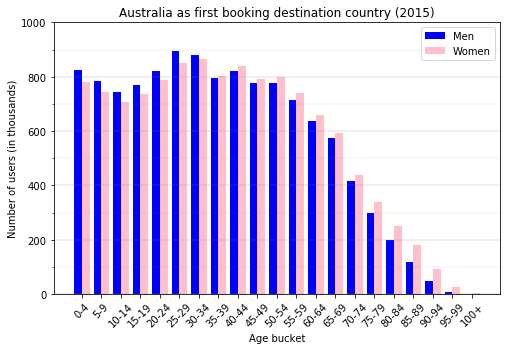
\includegraphics[scale=0.35]{../graphs/age_gender_bkts_AU}
\caption{Australia, $1$st booking destination ($2015$)}
\label{fig:australia}
\end{figure}

\begin{figure}[H]
\centering
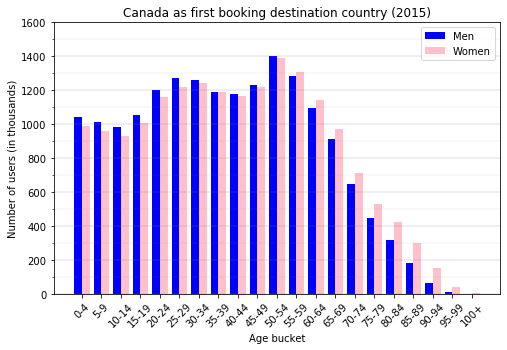
\includegraphics[scale=0.35]{../graphs/age_gender_bkts_CA}
\caption{Canada, $1$st booking destination ($2015$)}
\label{fig:canada}
\end{figure}

\begin{figure}[H]
\centering
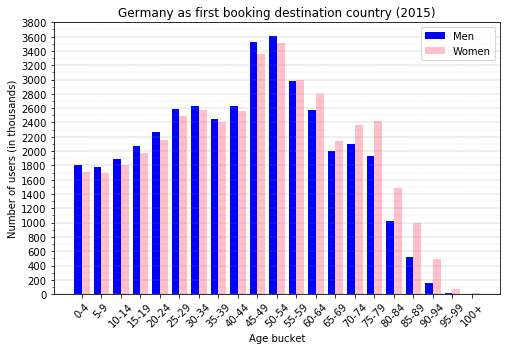
\includegraphics[scale=0.35]{../graphs/age_gender_bkts_DE}
\caption{Germany, $1$st booking destination ($2015$)}
\label{fig:germany}
\end{figure}

\begin{figure}[H]
\centering
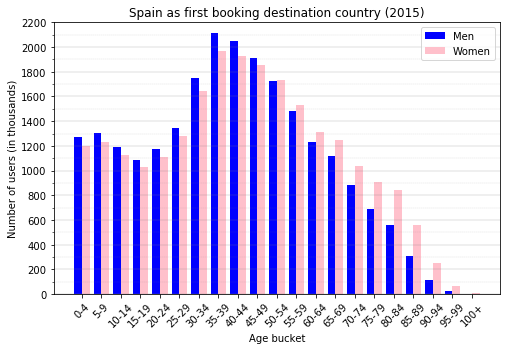
\includegraphics[scale=0.35]{../graphs/age_gender_bkts_ES}
\caption{Spain, $1$st booking destination ($2015$)}
\label{fig:spain}
\end{figure}

\begin{figure}[H]
\centering
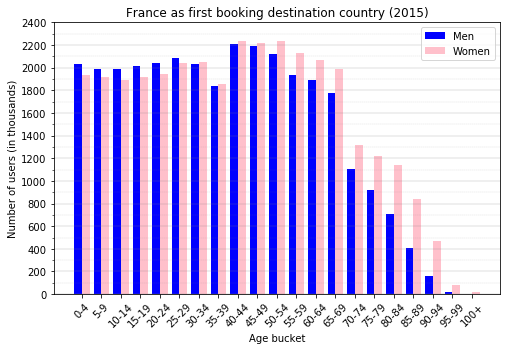
\includegraphics[scale=0.35]{../graphs/age_gender_bkts_FR}
\caption{France, $1$st booking destination ($2015$)}
\label{fig:france}
\end{figure}

\begin{figure}[H]
\centering
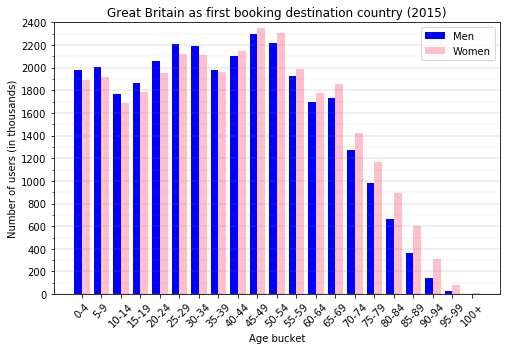
\includegraphics[scale=0.35]{../graphs/age_gender_bkts_GB}
\caption{Great Britain, $1$st booking destination ($2015$)}
\label{fig:greatbritain}
\end{figure}

\begin{figure}[H]
\centering
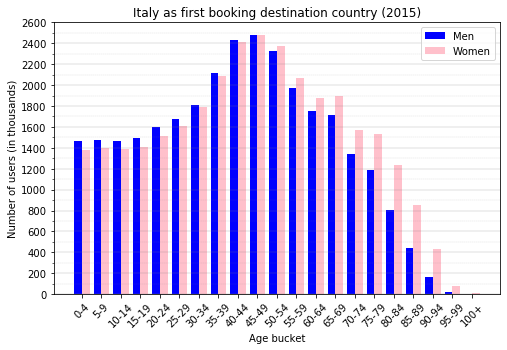
\includegraphics[scale=0.35]{../graphs/age_gender_bkts_IT}
\caption{Italy, $1$st booking destination ($2015$)}
\label{fig:italy}
\end{figure}

\begin{figure}[H]
\centering
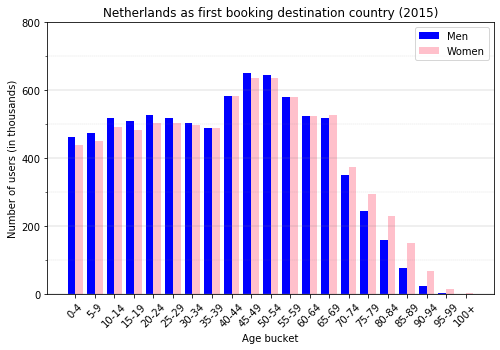
\includegraphics[scale=0.35]{../graphs/age_gender_bkts_NL}
\caption{Netherlands, $1$st booking destination ($2015$)}
\label{fig:netherlands}
\end{figure}

\begin{figure}[H]
\centering
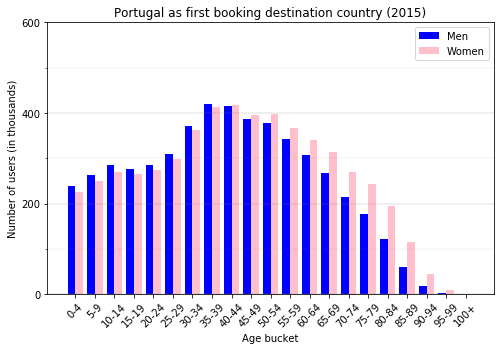
\includegraphics[scale=0.35]{../graphs/age_gender_bkts_PT}
\caption{Portugal, $1$st booking destination ($2015$)}
\label{fig:portugal}
\end{figure}

\begin{figure}[H]
\centering
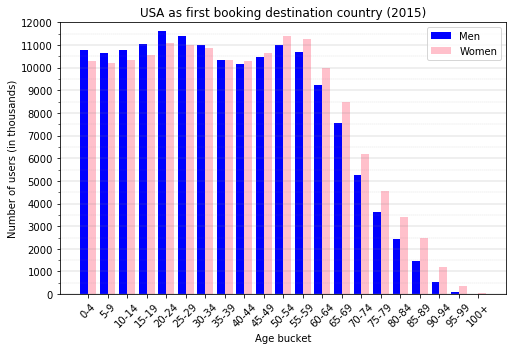
\includegraphics[scale=0.35]{../graphs/age_gender_bkts_US}
\caption{USA, $1$st booking destination ($2015$)}
\label{fig:usa}
\end{figure}

\subsubsection{\textit{countries.csv}}

In this second tabular data file, $3$ elements seem interessant to observe:
\begin{itemize}
\item The distance between each possible first booking destination country for Airbnb's panel new users and the USA (see Figure \ref{fig:km});
\item The area of each possible first booking destination country for Airbnb's panel new users (see Figure \ref{fig:km2});
\item The Levenshtein distance between the language of each possible first booking destination country for Airbnb's panel new users and the USA language (see Figure \ref{fig:language}).
\end{itemize}

\begin{figure}[H]
\centering
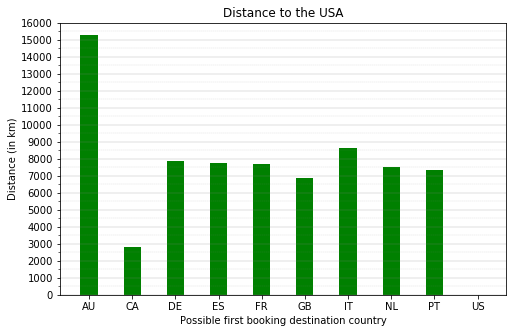
\includegraphics[scale=0.35]{../graphs/countries_distance_km}
\caption{Distance to the USA (in $km$)}
\label{fig:km}
\end{figure}

\begin{figure}[H]
\centering
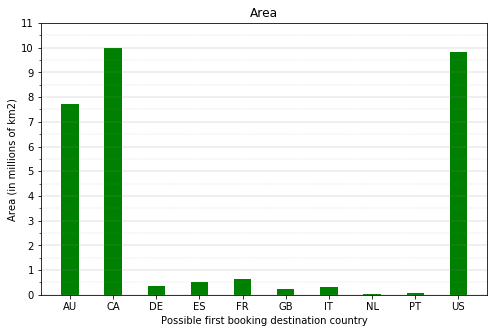
\includegraphics[scale=0.35]{../graphs/countries_destination_km2}
\caption{Area (in millions of $km^{2}$)}
\label{fig:km2}
\end{figure}

\begin{figure}[H]
\centering
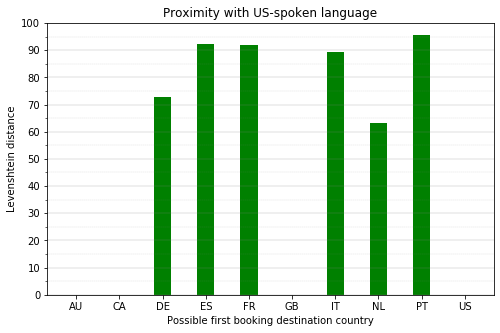
\includegraphics[scale=0.35]{../graphs/countries_language_levenshtein_distance}
\caption{Proximity with US-spoken language}
\label{fig:language}
\end{figure}

\subsubsection{\textit{train\_users\_2.csv}}

In this third---and last---tabular data file, as major information, it can be noted that it is structured around $213,451$ Airbnb's new users, with a first booking destination country repartition (see Figure \ref{fig:repartition}) as it can be observed in Table \ref{tab:repartition}:

\begin{table}[H]
\caption{First booking destination country repartition}
\centering
\begin{tabular}{ll}
\toprule
Country & Number of users \\
\midrule
No Destination Found & $124,543$ \\
USA & $62,376$ \\
Other & $10,094$ \\
France & $5,023$ \\
Italy & $2,835$ \\
Great Britain & $2,324$ \\
Spain & $2,249$ \\
Canada & $1,428$ \\
Germany & $1,061$ \\
Netherlands & $762$ \\
Australia & $539$ \\
Portugal & $217$ \\
\bottomrule
\end{tabular}
\label{tab:repartition}
\end{table}

Clearly, for the target variable of our problem for this study, the dataset classes are imbalanced, which is, by far, not the best situation.

\begin{figure}[H]
\centering
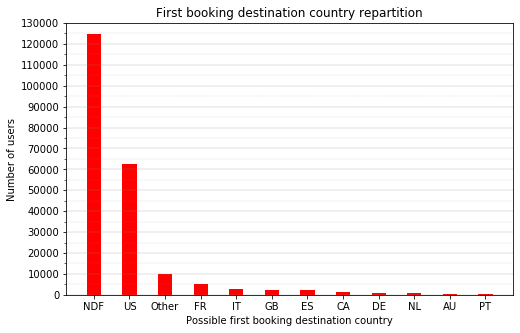
\includegraphics[scale=0.35]{../graphs/train_users_2_country_destination}
\caption{First booking destination country repartition}
\label{fig:repartition}
\end{figure}

As complementary information extracted in this tabular data file, the following can be visualized:
\begin{itemize}
\item The account creation dates for Airbnb's panel new users (see Figure \ref{fig:account});
\item The age repartition of Airbnb's panel new users (see Figure \ref{fig:age});
\item The gender repartition of Airbnb's panel new users (see Figure \ref{fig:gender}).
\end{itemize}

\begin{figure}[H]
\centering
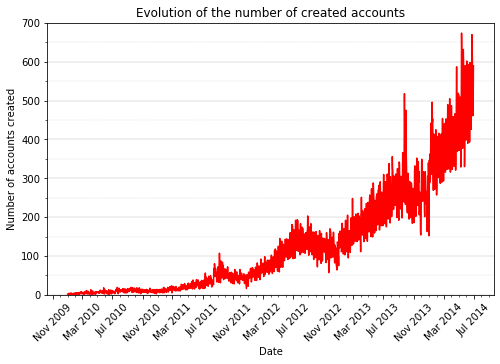
\includegraphics[scale=0.35]{../graphs/train_users_2_date_account_created}
\caption{Evolution of the number of created accounts}
\label{fig:account}
\end{figure}

\begin{figure}[H]
\centering
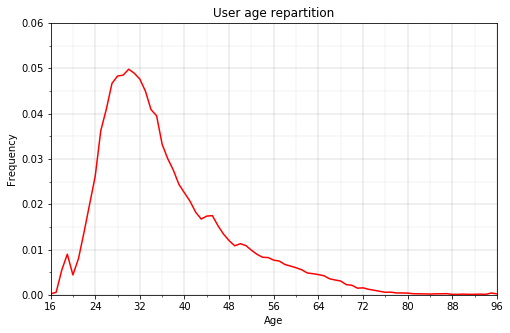
\includegraphics[scale=0.35]{../graphs/train_users_2_age}
\caption{User age repartition}
\label{fig:age}
\end{figure}

\begin{figure}[H]
\centering
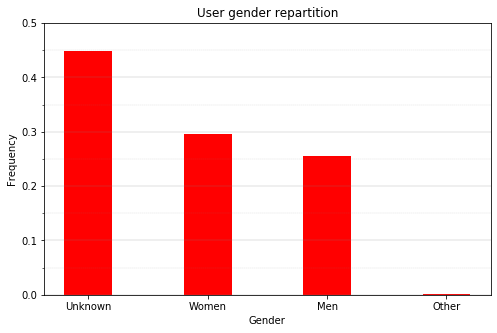
\includegraphics[scale=0.35]{../graphs/train_users_2_gender}
\caption{User gender repartition}
\label{fig:gender}
\end{figure}

\subsection{Analysis}

Respectively to \textit{age\_gender\_bkts.csv}, which lists, for the year $2015$, the volume of new users who have chosen between $10$ possible destination countries (Australia, Canada, Germany, Spain, France, Great Britain, Italy, Netherlands, Portugal and USA) as their first Airbnb booking, segmented by gender and age repartition, $3$ main conclusions can be made:
\begin{itemize}
\item Firstly, in the Airbnb's panel new users, there is an important variation between volumetries of travellers corresponding to each first booking destination country, with important proportions for the USA and a marked difference between this destination and the second in the list (Germany);
\item Secondly, it appears that within each possible first booking destination country, for each age bucket, there is no significative difference between volumetries of travellers corresponding each one of the two genders (nevertheless, it can be noticed that, approximately from $75$ years old, the proportion of women within travellers tends to become impacting, independently from the first booking destination country, element which can probably be put in relation with a life expectancy more important for women than for men in the USA, country from where Airbnb's panel new users come from).
\item Thirdly, we can report that approximately from $50$ years old, the volumetries of travellers for each possible first booking destination country tend to tumble down significantly.
\end{itemize}

Respectively to \textit{countries.csv}, which lists some characteristics of each possible first booking destination country for Airbnb's panel new users, once again, $3$ main conclusions can be made:
\begin{itemize}
\item Firstly, within the possible first booking destination countries, we can note $4$ categories corresponding to the distance to the USA: The USA itself, Canada which is a border country, the European countries (Germany, Spain, France, Great Britain, Italy, Netherlands and Portugal), and, finally, Australia, the most distant country. We can conjecture that the nearest countries to the USA (and the USA itself per se) are going to be favored by the Airbnb's panel new users, taking into account that they come from the USA.
\item Secondly, in respect to the areas of each possible first booking destination country, we can consider $2$ main categories: A a first category of "big" countries (USA, Canada and Australia), and a second one of "small" countries (the European ones, Germany, Spain, France, Great Britain, Italy, Netherlands and Portugal). It's difficult to make assumptions on this aspect: Indeed, a country like Australia has an important part of its area that is desert or semi-arid (the center of the country) meanwhile the European countries, despite their "small" areas, are reputed for their touristic attractivity.
\item Thirdly, considering the Levenshtein distance between the language of each possible first booking destination country and the USA language, we can note $3$ categories: English-speaking countries (The USA itself, Great Britain, Canada and Australia), Germanic-language-speaking countries (Germany and Netherlands) and Latin-language-speaking countries (Spain, France, Italy and Portugal). Here, we can make the assumption that English-speaking countries will be favored, then Germanic-language-speaking countries, and then Latin-language-speaking countries, by the Airbnb's panel new users, taking into account that they come from the USA.
\end{itemize}

\subsection{Preprocessing}

With an enhanced comprehension of the situation involved in the challenge, a better idea about Airbnb's user profiles, and now a clear vision of the positionment and ranking in users mind of each possible first booking destination country, we can now explain how we are going to preprocess the tabular data file \textit{train\_users\_2.csv}, which is going to be the main base to construct the future training and testing sets we will use to build our prediction models:
\begin{enumerate}
\item The target variable necessary for this project is clearly identified: \textit{country\_destination}.
\item We will perform some checks on the \textit{id} variable to make sure no error is present (we need to check that only unique ids can be counted), and then, we will drop this feature (it is not relevant for our study).
\item The \textit{age} feature needs to be treated to eliminate outliers.
\item All missing values (\textit{NaN} values) and imprecise values (e.g., \textit{-unknown-}) will need to be treated carefully for each impacted variable: More precisely, we are going to drop the variable \textit{date\_first\_booking} because it counts too numerous missing values, concerning the variable \textit{age}, we will treat missing values as outliers, and replace them by $-1$, and, lastly, for the variable \textit{first\_affiliate\_tracked}, missing values will be replaced by \textit{untracked}, creating this way a new category inside the variable. Then, in order to "penalize" imprecise values (features \textit{gender} and \textit{first\_browser} counts some \textit{-unknown-} values) and now transformed missing values (i.e., features \textit{age} and \textit{first\_affiliate\_tracked}), we are going to create a new variable, \textit{nans}, which counts the total number of these occurrences, and add it to the dataset.
\item We need to transform the date features: \textit{date\_account\_created}, \textit{timestamp\_first\_active} and \textit{date\_first\_booking}, and, too, we will create a new variable based on dates, \textit{time\_lag}, the time lag between first activity date and account creation date for a given Airbnb new user.
\item We will need to handle the categorical features: \textit{gender}, \textit{signup\_method}, \textit{language}, \textit{affiliate\_channel}, \textit{affiliate\_provider}, \textit{first\_affiliate\_tracked}, \textit{signup\_app}, \textit{first\_device\_type} and \textit{first\_browser} (we will equally need to treat \textit{signup\_flow} as a categorical feature, though it contains numeric values, as these ones correspond to categories).
\item Lastly, we will need to scale the continuous variables we are going to introduce: \textit{nans}, the number of missing values and unprecise values for a given Airbnb new user, and \textit{time\_lag}, the time lag, for a given Airbnb new user, between first activity date and account creation date.
\end{enumerate}

Preprocessing the tabular data file this way, we get a consolidated dataset---to split between a training set ($80\%$) and a testing set ($20\%$) in a stratified mode to handle the problem of the imbalanced classes---composed by $213,451$ data points with $160$ feature variables, $1$ target variable each, and, more globally, $0$ missing values.

%% Problem Modeling %%

\section{Problem Modeling}

\subsection{General Methodology}

To build a prediction solution able to tackle the problem proposed in this challenge, as this is naturally implied, we are going to construct machine learning classifier models thanks to a supervised learning approach relying on the training and testing sets formed from the preprocessing of the tabular data file \textit{train\_users\_2.csv}.

As it has been specified, we will evaluate these various models we are going to build thanks to the \textit{normalized Discounted Cumulative Gain (normalized DCG)} quality metric, and we will benchmark them and consider their performance using a naive predictor as reference.

Below, we are going to follow $3$ main approches to try to solve the challenge's problem:
\begin{itemize}
\item Firstly, we will adopt a global approach of the situation, handling all the first booking destination country classes at the same time, discarding the fact that they are widely imbalanced.
\item Secondly, we will still adopt a global approach of the situation, but this time, we will add $1$ step, building a new machine learning classifier model on the predictions proposed by the first machine learning classifier model, trying this way a correction step, with the aim to catch patterns on first model predictions to improve them.
\item Thirdly, trying to handle better the widely imbalanced first booking destination country classes, we will propose a pipeline of $4$ machine learning classifier models, and check if this approach is satisfying in comparison with a global approach of the situation.
\end{itemize}

Finally, we will analyse the results and propose a solution to the challenge's problem.

\subsection{Naive Predictor}

To benchmark the prediction models we will build, here, as reference, we are going to consider a naive predictor: For each prediction it has to perform, it returns the following list of classified first booking destination country possibilities:

\{"NDF", "US", "other", "FR", "IT"\}

As it has been observed, this list corresponds to the ordered top 5 first booking destination country possibilities in the consolidated dataset considered in this project.

Below, in Table \ref{tab:naive}, we can observe the main results obtained with this naive predictor:

\begin{table}[H]
\caption{Naive predictor \textit{nDCG} mean scores}
\centering
\begin{tabular}{lll}
\toprule
Set & & \textit{nDCG} mean score \\
\midrule
training & global & $0.806766$ \\
testing & global & $0.806763$ \\
& Australia & $0.000000$ \\
& Canada & $0.000000$ \\
& Germany & $0.000000$ \\
& Spain & $0.000000$ \\
& France & $0.430677$ \\
& Great Britain & $0.000000$ \\
& Italy & $0.386853$ \\
& NDF & $1.000000$ \\
& Netherlands & $0.000000$ \\
& Portugal & $0.000000$ \\
& USA & $0.630930$ \\
& other & $0.500000$ \\
\bottomrule
\end{tabular}
\label{tab:naive}
\end{table}

\subsection{Global Approach of the Situation}

For the global approach of the situation which has been explained above, we have tried $6$ types of classifier models.

\subsubsection{Random Forest Classifier}

The first family of models we have mobilized to tackle, with a global approach of the situation, the problem proposed in the challenge, is the family of random forest classifiers (see \cite{Ho_1995}).

As precised in Scikit-Learn's documentation, we can note that:

\textit{"A random forest is a meta estimator that fits a number of decision tree classifiers on various sub-samples of the dataset and uses averaging to improve the predictive accuracy and control over-fitting."}

\textit{"Each tree in the ensemble is built from a sample drawn with replacement (i.e., a bootstrap sample) from the training set. Furthermore, when splitting each node during the construction of a tree, the best split is found either from all input features or a random subset."}

\textit{"The purpose of these two sources of randomness is to decrease the variance of the forest estimator. Indeed, individual decision trees typically exhibit high variance and tend to overfit. The injected randomness in forests yield decision trees with somewhat decoupled prediction errors. By taking an average of those predictions, some errors can cancel out. Random forests achieve a reduced variance by combining diverse trees, sometimes at the cost of a slight increase in bias. In practice the variance reduction is often significant hence yielding an overall better model."}

Performing a random search to tune hyperparameters, we have found that, for a random forest classifier, the best\footnote{This qualifier has to be considered as relative, considering the fact that the hardware at our disposal for the project had very limited computation capabilities.} tuning of key hyperparameters is as expressed in the following Table \ref{tab:rfchyp}:

\begin{table}[H]
\caption{Random forest classifier best key hyperparameters}
\centering
\begin{tabular}{ll}
\toprule
Number of trees in the forest & $77$ \\
Min number of samples to split internal node & $10$ \\
Min number of samples to be at a leaf node & $1$ \\
Max depth of the tree & Pure leaves \\
Weighted classes & Yes \\
Whole datset is used to build each tree & Yes \\
\bottomrule
\end{tabular}
\label{tab:rfchyp}
\end{table}

Below, in Table \ref{tab:rfc}, we can observe the main results obtained with such random forest classifier:

\begin{table}[H]
\caption{Best random forest classifier \textit{nDCG} mean scores}
\centering
\begin{tabular}{lll}
\toprule
Set & & \textit{nDCG} mean score \\
\midrule
training & global & $0.906901$ \\
testing & global & $0.816485$ \\
& Australia & $0.007164$ \\
& Canada & $0.035858$ \\
& Germany & $0.023998$ \\
& Spain & $0.106723$ \\
& France & $0.375889$ \\
& Great Britain & $0.111050$ \\
& Italy & $0.166975$ \\
& NDF & $0.965516$ \\
& Netherlands & $0.013758$ \\
& Portugal & $0.000000$ \\
& USA & $0.742169$ \\
& other & $0.474328$ \\
\bottomrule
\end{tabular}
\label{tab:rfc}
\end{table}

\subsubsection{Adaptive Boosting Classifier}

The second family of models we have mobilized to tackle, with a global approach of the situation, the problem proposed in the challenge, is the family of adaptive boosting classifiers (see \cite{Freund_1997}).

As precised in Scikit-Learn's documentation, we can note that:

\textit{"An AdaBoost classifier is a meta-estimator that begins by fitting a classifier on the original dataset and then fits additional copies of the classifier on the same dataset but where the weights of incorrectly classified instances are adjusted such that subsequent classifiers focus more on difficult cases."}

\textit{"The core principle of AdaBoost is to fit a sequence of weak learners (i.e., models that are only slightly better than random guessing, such as small decision trees) on repeatedly modified versions of the data. The predictions from all of them are then combined through a weighted majority vote (or sum) to produce the final prediction. The data modifications at each so-called boosting iteration consist of applying weights $w_1$, $w_2$, \ldots, $w_N$ to each of the training samples. Initially, those weights are all set to $w_i = \frac{1}{N}$, so that the first step simply trains a weak learner on the original data. For each successive iteration, the sample weights are individually modified and the learning algorithm is reapplied to the reweighted data. At a given step, those training examples that were incorrectly predicted by the boosted model induced at the previous step have their weights increased, whereas the weights are decreased for those that were predicted correctly. As iterations proceed, examples that are difficult to predict receive ever-increasing influence. Each subsequent weak learner is thereby forced to concentrate on the examples that are missed by the previous ones in the sequence."}

Performing a random search to tune hyperparameters, we have found that, for an adaptive boosting classifier, the best tuning of key hyperparameters is as expressed in the following Table \ref{tab:abchyp}:

\begin{table}[H]
\caption{Adaptive boosting classifier best key hyperparameters}
\centering
\begin{tabular}{ll}
\toprule
Max number of estimators (for terminated boosting) & $70$ \\
Learning rate & $1.0$ \\
\bottomrule
\end{tabular}
\label{tab:abchyp}
\end{table}

Below, in Table \ref{tab:abc}, we can observe the main results obtained with such adaptive boosting classifier:

\begin{table}[H]
\caption{Best adaptive boosting classifier \textit{nDCG} mean scores}
\centering
\begin{tabular}{lll}
\toprule
Set & & \textit{nDCG} mean score \\
\midrule
training & global & $0.823412$ \\
testing & global & $0.821829$ \\
& Australia & $0.000000$ \\
& Canada & $0.017891$ \\
& Germany & $0.012309$ \\
& Spain & $0.088466$ \\
& France & $0.434981$ \\
& Great Britain & $0.067387$ \\
& Italy & $0.233823$ \\
& NDF & $0.949711$ \\
& Netherlands & $0.002545$ \\
& Portugal & $0.000000$ \\
& USA & $0.783837$ \\
& other & $0.495794$ \\
\bottomrule
\end{tabular}
\label{tab:abc}
\end{table}

\subsubsection{Extra-Trees Classifier}

The third family of models we have mobilized to tackle, with a global approach of the situation, the problem proposed in the challenge, is the family of extra-trees classifiers (see \cite{Geurts_2006}).

As precised in Scikit-Learn's documentation, we can note that:

\textit{"An extra-trees classifier is a meta estimator that fits a number of randomized decision trees (a.k.a. extra-trees) on various sub-samples of the dataset and uses averaging to improve the predictive accuracy and control over-fitting."}

\textit{"In extremely randomized trees, randomness goes one step further in the way splits are computed. As in random forests, a random subset of candidate features is used, but instead of looking for the most discriminative thresholds, thresholds are drawn at random for each candidate feature and the best of these randomly-generated thresholds is picked as the splitting rule. This usually allows to reduce the variance of the model a bit more, at the expense of a slightly greater increase in bias."}

Performing a random search to tune hyperparameters, we have found that, for an extra-trees classifier, the best tuning of key hyperparameters is as expressed in the following Table \ref{tab:etchyp}:

\begin{table}[H]
\caption{Extra-trees classifier best key hyperparameters}
\centering
\begin{tabular}{ll}
\toprule
Number of trees in the forest & $55$ \\
Min number of samples to split an internal node & $10$ \\
Min number of samples to be at a leaf node & $1$ \\
Max depth of the tree & $100$ \\
Weighted classes & Yes \\
Whole datset is used to build each tree & Yes \\
\bottomrule
\end{tabular}
\label{tab:etchyp}
\end{table}

Below, in Table \ref{tab:etc}, we can observe the main results obtained with such extra-trees classifier:

\begin{table}[H]
\caption{Best extra-trees classifier \textit{nDCG} mean scores}
\centering
\begin{tabular}{lll}
\toprule
Set & & \textit{nDCG} mean score \\
\midrule
training & global & $0.882097$ \\
testing & global & $0.813936$ \\
& Australia & $0.007570$ \\
& Canada & $0.040835$ \\
& Germany & $0.025496$ \\
& Spain & $0.133674$ \\
& France & $0.350670$ \\
& Great Britain & $0.111953$ \\
& Italy & $0.165946$ \\
& NDF & $0.975789$ \\
& Netherlands & $0.013014$ \\
& Portugal & $0.000000$ \\
& USA & $0.715075$ \\
& other & $0.466886$ \\
\bottomrule
\end{tabular}
\label{tab:etc}
\end{table}

\subsubsection{Gradient Boosting Classifier}

The fourth family of models we have mobilized to tackle, with a global approach of the situation, the problem proposed in the challenge, is the family of gradient boosting classifiers (see \cite{Breiman_1997}).

As precised in Scikit-Learn's documentation, we can note that:

\textit{"Gradient Tree Boosting or Gradient Boosted Regression Trees (GBRT) is a generalization of boosting to arbitrary differentiable loss functions. GBRT is an accurate and effective off-the-shelf procedure that can be used for both regression and classification problems."}

\textit{"The advantages of GBRT are natural handling of data of mixed type (heterogeneous features), predictive power and robustness to outliers in output space (via robust loss functions), while the disadvantages of GBRT are scalability, due to the sequential nature of boosting it can hardly be parallelized."}

Due to the fact that the hardware at our disposal for the project had very limited computation capabilities, we have not been able to tune the keys hyperparameters that define these classifiers\footnote{The fine tuning of the numerous hyperparameters that can set gradient boosting classifiers has a very high cost in terms of computation capabilities.}.

Below, in Table \ref{tab:gbc}, we can observe the main results obtained with an \textit{out-of-the-box} boosting classifier:

\begin{table}[H]
\caption{\textit{Out-of-the-box} gradient boosting classifier \textit{nDCG} mean scores}
\centering
\begin{tabular}{lll}
\toprule
Set & & \textit{nDCG} mean score \\
\midrule
training & global & $0.830643$ \\
testing & global & $0.824181$ \\
& Australia & $0.003988$ \\
& Canada & $0.018133$ \\
& Germany & $0.014461$ \\
& Spain & $0.100437$ \\
& France & $0.432548$ \\
& Great Britain & $0.084488$ \\
& Italy & $0.225514$ \\
& NDF & $0.946023$ \\
& Netherlands & $0.006696$ \\
& Portugal & $0.000000$ \\
& USA & $0.798475$ \\
& other & $0.496727$ \\
\bottomrule
\end{tabular}
\label{tab:gbc}
\end{table}

\subsubsection{Multi-Layer Perceptron Classifier}

The fifth family of models we have mobilized to tackle, with a global approach of the situation, the problem proposed in the challenge, is the family of multi-layer perceptron classifiers (see \cite{Hinton_1990}).

As precised in Scikit-Learn's documentation, we can note that:

\textit{"Multi-layer Perceptron (MLP) is a supervised learning algorithm that learns a function $f : \mathbb{R}^m \longrightarrow \mathbb{R}$ by training on a dataset, where $m$ is the number of dimensions for input and $1$ is the number of dimensions for output. Given a set of features $X = x_1, x_2, \ldots x_m$ and a target $y$, it can learn a non-linear function approximator for either classification or regression."}

\textit{"The advantages of Multi-layer Perceptron are capability to learn non-linear models and capability to learn models in real-time (on-line learning), while the disadvantages of Multi-layer Perceptron (MLP) include MLP with hidden layers have a non-convex loss function where there exists more than one local minimum (therefore different random weight initializations can lead to different validation accuracy), MLP requires tuning a number of hyperparameters such as the number of hidden neurons, layers, and iterations, and MLP is sensitive to feature scaling."}

Performing a random search to tune hyperparameters, we have found that, for a multi-layer perceptron classifier, the best tuning of key hyperparameters is as expressed in the following Table \ref{tab:mlpchyp}:

\begin{table}[H]
\caption{Multi-layer perceptron classifier best key hyperparameters}
\centering
\begin{tabular}{ll}
\toprule
Training data proportion for validation set & $20\%$ \\
Solver & Adam \\
Max number of epochs without improvement & $10$ \\
Max number of iterations & $200$ \\
Initial learning rate & $0.0001$ \\
Number of neurons by hidden layers & $80$, $40$, $20$ \\
Early stopping & Yes \\
Activation function & ReLU \\
\bottomrule
\end{tabular}
\label{tab:mlpchyp}
\end{table}

Below, in Table \ref{tab:mlpc}, we can observe the main results obtained with such multi-layer perceptron classifier:

\begin{table}[H]
\caption{Best multi-layer perceptron classifier \textit{nDCG} mean scores}
\centering
\begin{tabular}{lll}
\toprule
Set & & \textit{nDCG} mean score \\
\midrule
training & global & $0.822968$ \\
testing & global & $0.822270$ \\
& Australia & $0.000000$ \\
& Canada & $0.000000$ \\
& Germany & $0.000000$ \\
& Spain & $0.413072$ \\
& France & $0.411407$ \\
& Great Britain & $0.000832$ \\
& Italy & $0.010234$ \\
& NDF & $0.935384$ \\
& Netherlands & $0.000000$ \\
& Portugal & $0.000000$ \\
& USA & $0.818191$ \\
& other & $0.491116$ \\
\bottomrule
\end{tabular}
\label{tab:mlpc}
\end{table}

\subsubsection{Voting Classifier}

The sixth---and last---family of models we have mobilized to tackle, with a global approach of the situation, the problem proposed in the challenge, is the family of voting classifiers, which allows, generally, to reach better results than the ones obtained by the classifiers on whose they are built (e.g., in another context, see \cite{VanHalteren_1998}).

In our study, we have built a voting classifier using the best random forest, gradient boosting and multi-layer perceptron classifiers presented above\footnote{Voting methods work all the better as the predictors on whose they are built are really independent from each other: In order to obtain sufficiently varied classifiers, one solution is to use very different training algorithms, this increases the chances that they make very different errors, thereby improving the accuracy of the set.}.

Below, in Table \ref{tab:vc}, we can observe the main results obtained with such voting classifier:

\begin{table}[H]
\caption{Voting classifier \textit{nDCG} mean scores}
\centering
\begin{tabular}{lll}
\toprule
Set & & \textit{nDCG} mean score \\
\midrule
training & global & $0.869396$ \\
testing & global & $0.823524$ \\
& Australia & $0.000000$ \\
& Canada & $0.006763$ \\
& Germany & $0.007919$ \\
& Spain & $0.328300$ \\
& France & $0.427147$ \\
& Great Britain & $0.018735$ \\
& Italy & $0.054544$ \\
& NDF & $0.948974$ \\
& Netherlands & $0.003289$ \\
& Portugal & $0.000000$ \\
& USA & $0.793151$ \\
& other & $0.497145$ \\
\bottomrule
\end{tabular}
\label{tab:vc}
\end{table}

\subsection{Stratified Global Approach of the Situation}

As a second attempt to tackle the problem presented in the challenge, we have, like for the first attempt, adopted a global approach of the situation, but this time, we have added $1$ step, building a new machine learning classifier model on the predictions proposed by the first machine learning classifier model, trying this way a correction step, with the aim to catch patterns on first model predictions to improve them.

As core machine learning classifier model, we have used the voting classifier presented above, and on its predictions on the training set, considered as probabilities for each first booking destination country class, we have built a gradient boosting classifier\footnote{The results obtained by this classifier, in comparison with the ones obtained by the other tried classifiers, led us to mobilize it, as it seems to handle better the data present in the consolidated dataset.} to try to correct them, and to propose this way corrected predictions.

Below, in Table \ref{tab:cvc}, we can observe the main results obtained with such corrected voting classifier:

\begin{table}[H]
\caption{Corrected voting classifier \textit{nDCG} mean scores}
\centering
\begin{tabular}{lll}
\toprule
Set & & \textit{nDCG} mean score \\
\midrule
training & global & $0.951813$ \\
testing & global & $0.780407$ \\
& Australia & $0.059779$ \\
& Canada & $0.078116$ \\
& Germany & $0.100146$ \\
& Spain & $0.231286$ \\
& France & $0.386274$ \\
& Great Britain & $0.125668$ \\
& Italy & $0.136344$ \\
& NDF & $0.887426$ \\
& Netherlands & $0.041941$ \\
& Portugal & $0.000000$ \\
& USA & $0.772363$ \\
& other & $0.441702$ \\
\bottomrule
\end{tabular}
\label{tab:cvc}
\end{table}

\subsection{Decomposed Approach of the Situation}

As a third attempt to tackle the problem presented in the challenge, we have tried to handle better the widely imbalanced first booking destination country classes, and for that, we have proposed a pipeline of $4$ machine learning classifier models, more precisely gradient boosting classifiers\footnote{As it has been noted previously, it seems that it is this type of classifiers which handle the best the data present in the consolidated dataset.}, structured around $4$ steps:
\begin{enumerate}
\item A first step where a first gradient boosting classifier will have the task to determine exclusively if the first booking destination country is "NDF".
\item If the prediction provided by this first gradient boosting classifier is different from "NDF", then, a second step will be performed, where a second gradient boosting classifier will have the task to determine exclusively if the first booking destination country is "USA".
\item If the prediction provided by this second gradient boosting classifier is different from "USA", then, a third step will be performed, where a third gradient boosting classifier will have the task to determine exclusively if the first booking destination country is "other".
\item Lastly, if the prediction provided by this third gradient boosting classifier is different from "other", then, a fourth step will be performed, where a fourth gradient boosting classifier will have the task to determine the first booking destination country among the remaining possibilities for first booking destination country ("FR", "IT", "GB", "ES", "CA", "DE", "NL", "AU" and "PT").
\end{enumerate}

Below, in Table \ref{tab:gbcp}, we can observe the main results obtained with such gradient boosting classifiers pipeline:

\begin{table}[H]
\caption{Gradient boosting classifiers pipeline \textit{nDCG} mean scores}
\centering
\begin{tabular}{lll}
\toprule
Set & & \textit{nDCG} mean score \\
\midrule
training & global & $0.823940$ \\
testing & global & $0.822982$ \\
& Australia & $0.000000$ \\
& Canada & $0.000000$ \\
& Germany & $0.002976$ \\
& Spain & $0.004444$ \\
& France & $0.433142$ \\
& Great Britain & $0.002001$ \\
& Italy & $0.388995$ \\
& NDF & $0.926442$ \\
& Netherlands & $0.000000$ \\
& Portugal & $0.000000$ \\
& USA & $0.832884$ \\
& other & $0.499009$ \\
\bottomrule
\end{tabular}
\label{tab:gbcp}
\end{table}

\subsection{Results Analysis}

To analyse the various results we have obtained and to be able, thus, to determine the best machine learning classifier model to tackle the problem proposed in the challenge, we need to consider the following criteria, by order of importance:
\begin{enumerate}
\item The \textit{nDCG} mean score on testing set (see Figure \ref{fig:ndcgtest});
\item The \textit{nDCG} mean score on testing set for each possible first booking destination country (see Figures \ref{fig:ndcgtestau}, \ref{fig:ndcgtestca}, \ref{fig:ndcgtestde}, \ref{fig:ndcgtestes}, \ref{fig:ndcgtestfr}, \ref{fig:ndcgtestgb}, \ref{fig:ndcgtestit}, \ref{fig:ndcgtestndf}, \ref{fig:ndcgtestnl}, \ref{fig:ndcgtestother}, \ref{fig:ndcgtestpt}, \ref{fig:ndcgtestus});
\item The \textit{nDCG} mean score on training set (see Figure \ref{fig:ndcgtrain}), principally to put in perspective with the \textit{nDCG} mean score on testing set, and observe if the various compared predictors are concerned by overfitting.
\end{enumerate}

\begin{figure}[H]
\centering
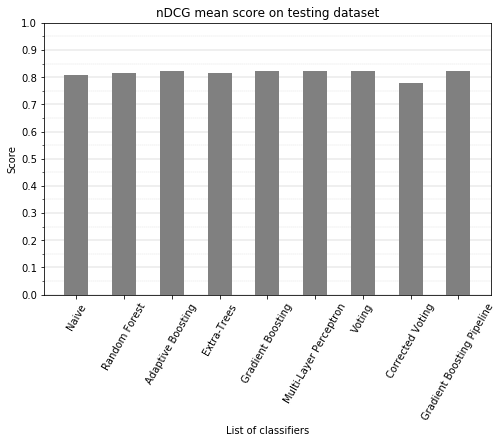
\includegraphics[scale=0.35]{../graphs/ndcg_mean_score_test}
\caption{Global \textit{nDCG} mean score on testing set}
\label{fig:ndcgtest}
\end{figure}

\begin{figure}[H]
\centering
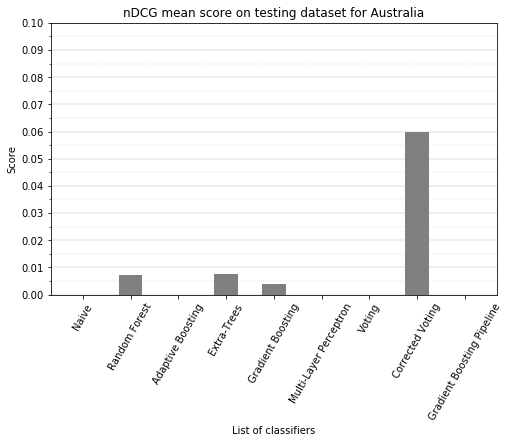
\includegraphics[scale=0.35]{../graphs/ndcg_mean_score_au_test}
\caption{Australia \textit{nDCG} mean score on testing set}
\label{fig:ndcgtestau}
\end{figure}

\begin{figure}[H]
\centering
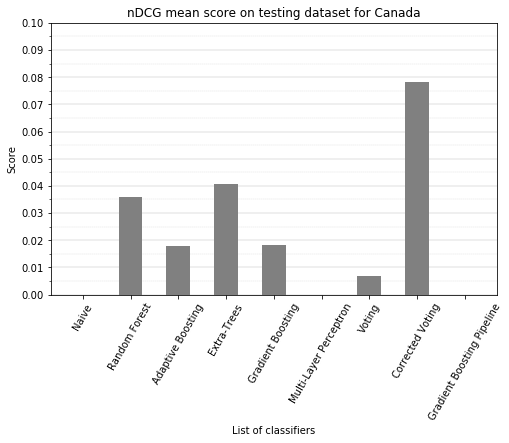
\includegraphics[scale=0.35]{../graphs/ndcg_mean_score_ca_test}
\caption{Canada \textit{nDCG} mean score on testing set}
\label{fig:ndcgtestca}
\end{figure}

\begin{figure}[H]
\centering
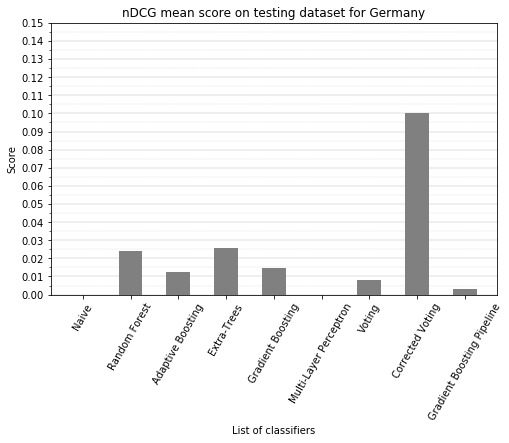
\includegraphics[scale=0.35]{../graphs/ndcg_mean_score_de_test}
\caption{Germany \textit{nDCG} mean score on testing set}
\label{fig:ndcgtestde}
\end{figure}

\begin{figure}[H]
\centering
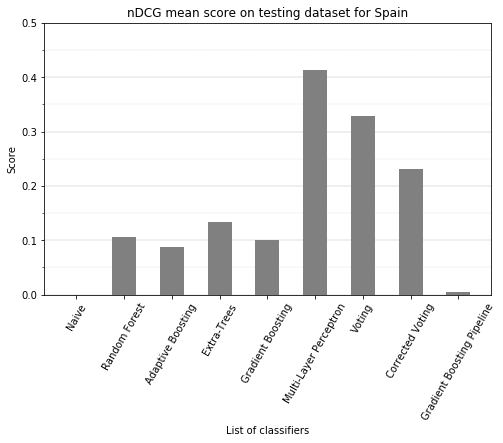
\includegraphics[scale=0.35]{../graphs/ndcg_mean_score_es_test}
\caption{Spain \textit{nDCG} mean score on testing set}
\label{fig:ndcgtestes}
\end{figure}

\begin{figure}[H]
\centering
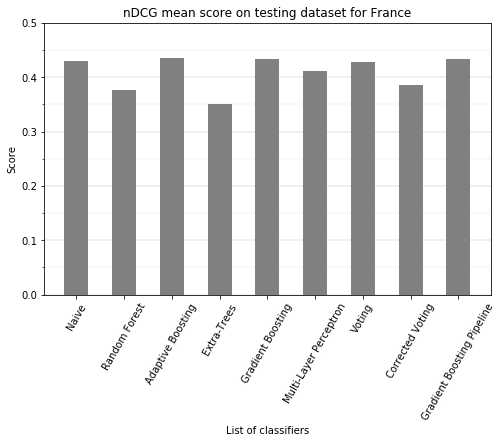
\includegraphics[scale=0.35]{../graphs/ndcg_mean_score_fr_test}
\caption{France \textit{nDCG} mean score on testing set}
\label{fig:ndcgtestfr}
\end{figure}

\begin{figure}[H]
\centering
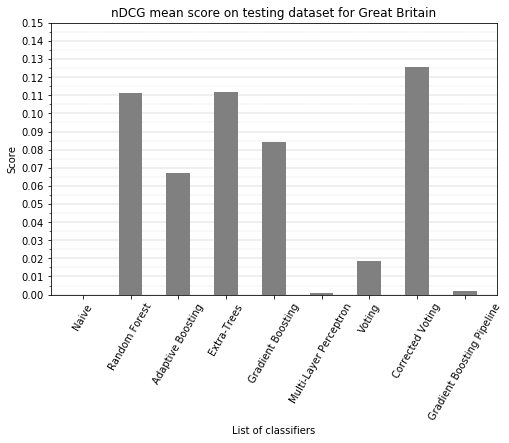
\includegraphics[scale=0.35]{../graphs/ndcg_mean_score_gb_test}
\caption{Great Britain \textit{nDCG} mean score on testing set}
\label{fig:ndcgtestgb}
\end{figure}

\begin{figure}[H]
\centering
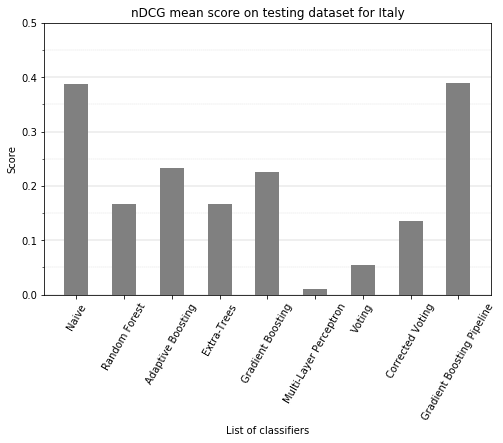
\includegraphics[scale=0.35]{../graphs/ndcg_mean_score_it_test}
\caption{Italy \textit{nDCG} mean score on testing set}
\label{fig:ndcgtestit}
\end{figure}

\begin{figure}[H]
\centering
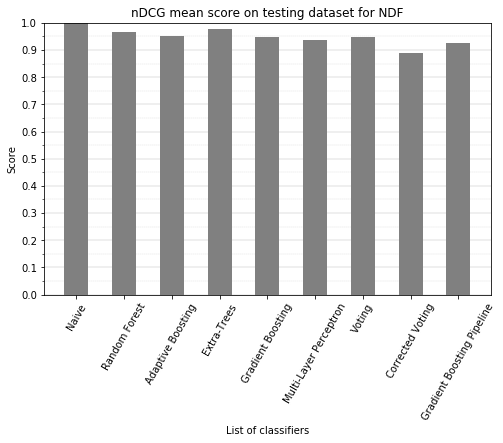
\includegraphics[scale=0.35]{../graphs/ndcg_mean_score_ndf_test}
\caption{NDF \textit{nDCG} mean score on testing set}
\label{fig:ndcgtestndf}
\end{figure}

\begin{figure}[H]
\centering
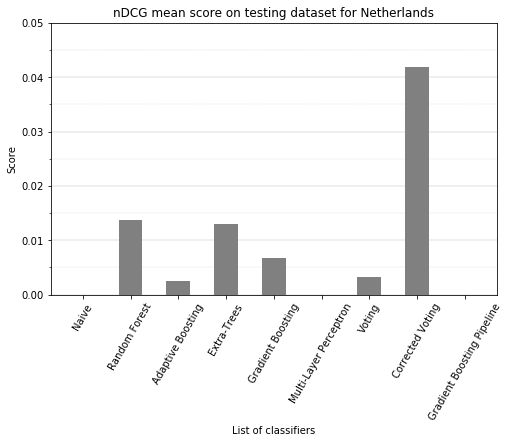
\includegraphics[scale=0.35]{../graphs/ndcg_mean_score_nl_test}
\caption{Netherlands \textit{nDCG} mean score on testing set}
\label{fig:ndcgtestnl}
\end{figure}

\begin{figure}[H]
\centering
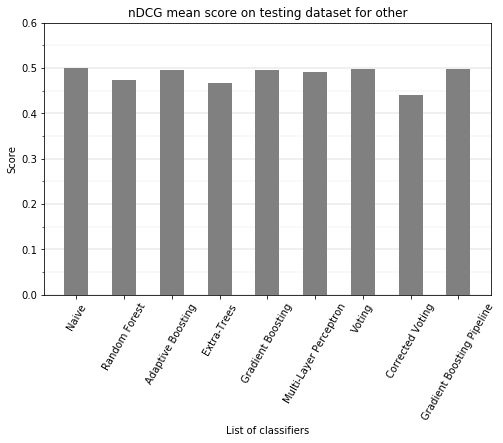
\includegraphics[scale=0.35]{../graphs/ndcg_mean_score_other_test}
\caption{Other \textit{nDCG} mean score on testing set}
\label{fig:ndcgtestother}
\end{figure}

\begin{figure}[H]
\centering
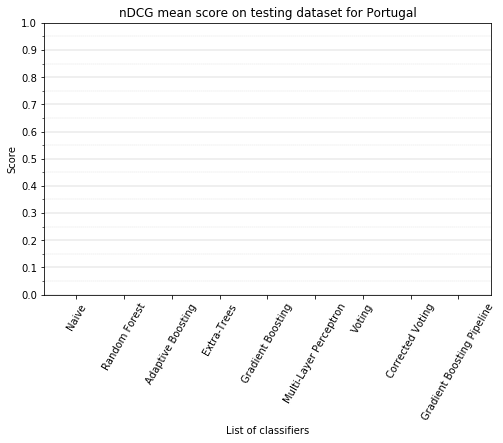
\includegraphics[scale=0.35]{../graphs/ndcg_mean_score_pt_test}
\caption{Portugal \textit{nDCG} mean score on testing set}
\label{fig:ndcgtestpt}
\end{figure}

\begin{figure}[H]
\centering
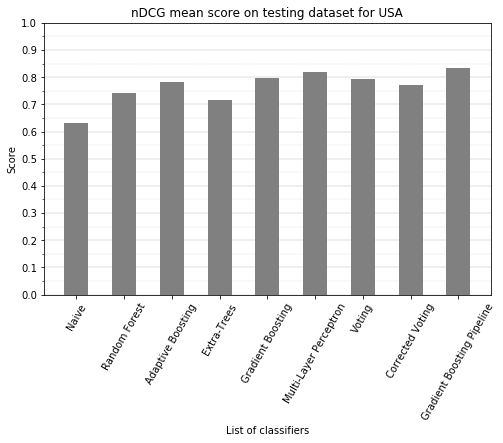
\includegraphics[scale=0.35]{../graphs/ndcg_mean_score_us_test}
\caption{USA \textit{nDCG} mean score on testing set}
\label{fig:ndcgtestus}
\end{figure}

\begin{figure}[H]
\centering
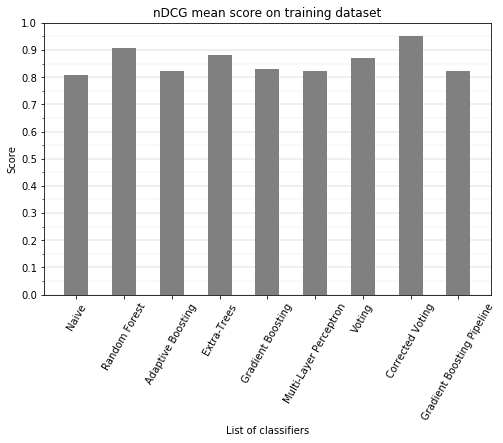
\includegraphics[scale=0.35]{../graphs/ndcg_mean_score_train}
\caption{Global \textit{nDCG} mean score on training set}
\label{fig:ndcgtrain}
\end{figure}

Respectively to the first criteria, we can note that the gradient boosting classifier we have built reaches the best \textit{nDCG} mean score on testing set, and if we compare it with the one obtained on training set, there no significative difference, and, thus, this classifier doesn't appear to be concerned by overfitting on the data considered in the context of the problem proposed by the challenge, which is clearly a good point.

Nonetheless, it is important, too, to remark that the \textit{nDCG} mean scores on testing set, for the classifier models we have built, are not significantly better than the one reached by the naive predictor, which constitutes a real concern.

In regards to the \textit{nDCG} mean scores on testing set for each possible first booking destination country, it appears very difficult to establish a clear hierarchy among the classifiers mobilized for this study. For sure, at least, it can be said that the situation is not a success, notably for underrepresented first booking destination country classes (e.g., none of the classifiers has been able to score points for Portugal as first booking destination): this imbalanced situation is really a tricky issue to handle. It is also interesting to note that the stratified global and decomposed approaches of the situation, specially designed for this characteristic of the problem, revealed themselves to be failures, presenting no real improvement in comparison with the global approach which has been firstly developed.

Respectively to this point, nevertheless, we can however note that the gradient boosting classifier that has been built has scored points for each one of the possible first booking destination, with the exception of Portugal, which is an indication that it has catched patterns in the data for each of these destinations, which is a good point, too.

%% Conclusion %%

\section{Proposed Solution}

With all the elements established during our study, and despite the weaknesses noticed in the previous subsection, naturally, we are led, to tackle the problem involved by the challenge, to propose a gradient boosting classifier, following a global approach of the situation, which has, furthermore, the benefit to constitute a simplified workflow in comparison with the $2$ other approaches we have explored too.

That being said, we can surmise $2$ main tracks to follow to try to improve the current results:
\begin{itemize}
\item In machine learning projects, the most import aspect, by far, is the data (e.g., an interested reader can consult \cite{Halevy_2009}). Here, the most tricky element about the data at our disposal is the widely imbalanced situation of the classes corresponding to the target variable. These situations are nevertheless not uncommon, and some methods can be followed to handle this situation (e.g., see \cite{Chawla_2002}). Finally, we can equally work on the dataset we have considered to build the various models we have tried, integrating the information contained in tabular data file \textit{sessions.csv}, and performing more feature engineering on the data (e.g., in tabular data file \textit{age\_gender\_bkts.csv}, it has been observed that users gender has no significative incidence on first booking destination country, regardeless of age buckets).
\item Concerning the gradient boosting classifier implemetation we have mobilized for this project, it would be an interesting idea to put in action the XGBoost implementation (see \cite{Chen_2016}), and, for that, it can be hoped to benefit from hardware with better computation capabilities than the ones we have benefited for our study, notably to set precisely the tuning of its hyperparameters, which is very costy in respect to these aspects.
\end{itemize}


%%%%%%%%%%%%%%%%%%%%%%%%%%%%%%%%%%%%%%%%%%%%%%%%%
%                BIBLIOGRAPHY                   %
%%%%%%%%%%%%%%%%%%%%%%%%%%%%%%%%%%%%%%%%%%%%%%%%%

\begin{normalsize}
\bibliography{references}
\end{normalsize}


%%%%%%%%%%%%%%%%%%%%%%%%%%%%%%%%%%%%%%%%%%%%%%%%%
%                     END                       %
%%%%%%%%%%%%%%%%%%%%%%%%%%%%%%%%%%%%%%%%%%%%%%%%%

\end{document}